\chapter{ANÁLISIS Y RESULTADOS}

\section{Análisis Exploratorio}
El centro poblado de Corpacancha cuenta con 177 casas, de las cuales 105 (59.3\%) están habitadas. Del censo realizado en 2018, se conoce que la población es de un total de 309 habitantes; de los cuales 141 (45.6\%) participaron en la campaña de salud. Tras haber realizado la limpieza correspondiente a los datos de la muestra proveniente del estudio VIRSEL, se conoce que la Hidatidosis Humana en el Centro poblado de Corpacancha tiene una prevalencia del 0.241 ($\pm$ 0.054 IC$_{95\%}$). Este estudio contó con una potencia estadística del 22.1 por ciento. La segunda campaña realizada junto al censo permitió aumentar la cobertura a un total de 196 participantes (63.4\%). Como resultado, la prevalencia disminuyó a 0.235 ($\pm$ 0.036 IC$_{95\%}$); indicando que la prevalencia del primer estudio se encontraba sobreestimada. Este estudio contó con una potencia estadística del 28.8 por ciento.

\newpage

\begin{figure}[h]\label{houses}
	\begin{center}
		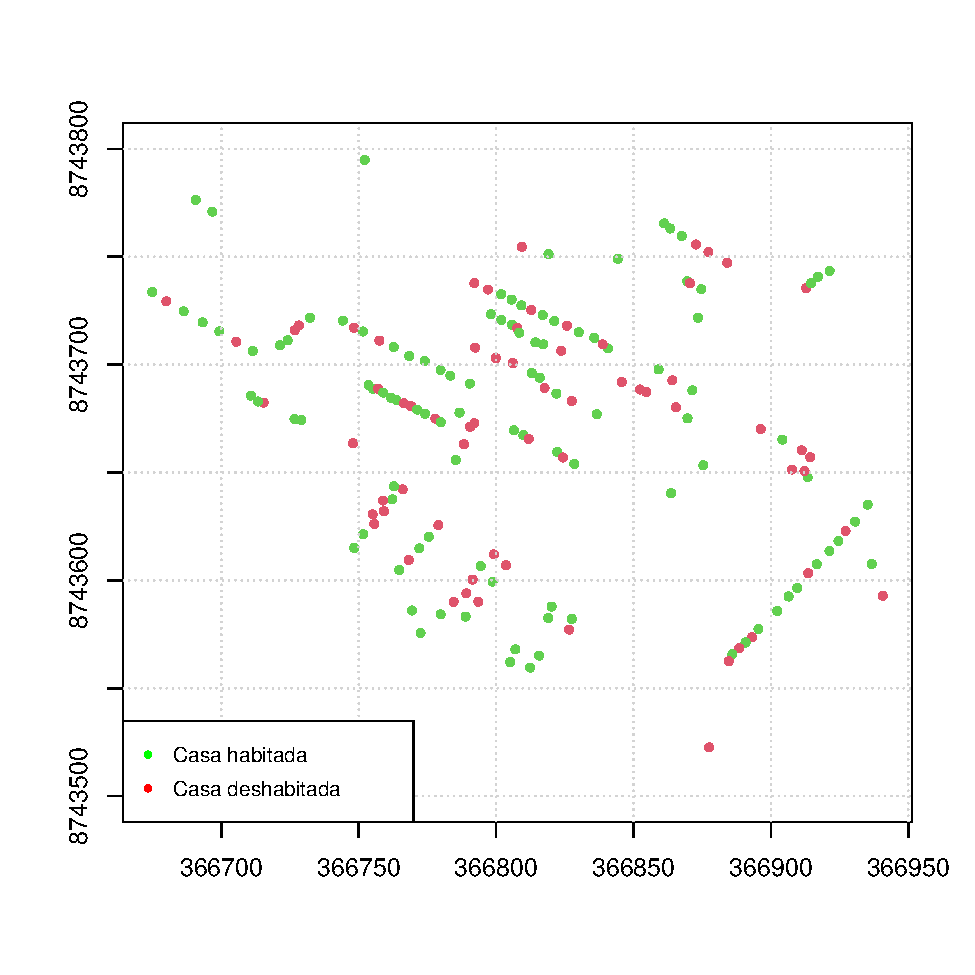
\includegraphics[width=0.85\textwidth]{graficos/houses.pdf}
	\end{center}
	\caption{Distribución en el espacio de las casas en el centro poblado de Corpacancha.}
\end{figure}

\newpage

\begin{figure}[h]\label{houses_participation}
	\begin{center}
		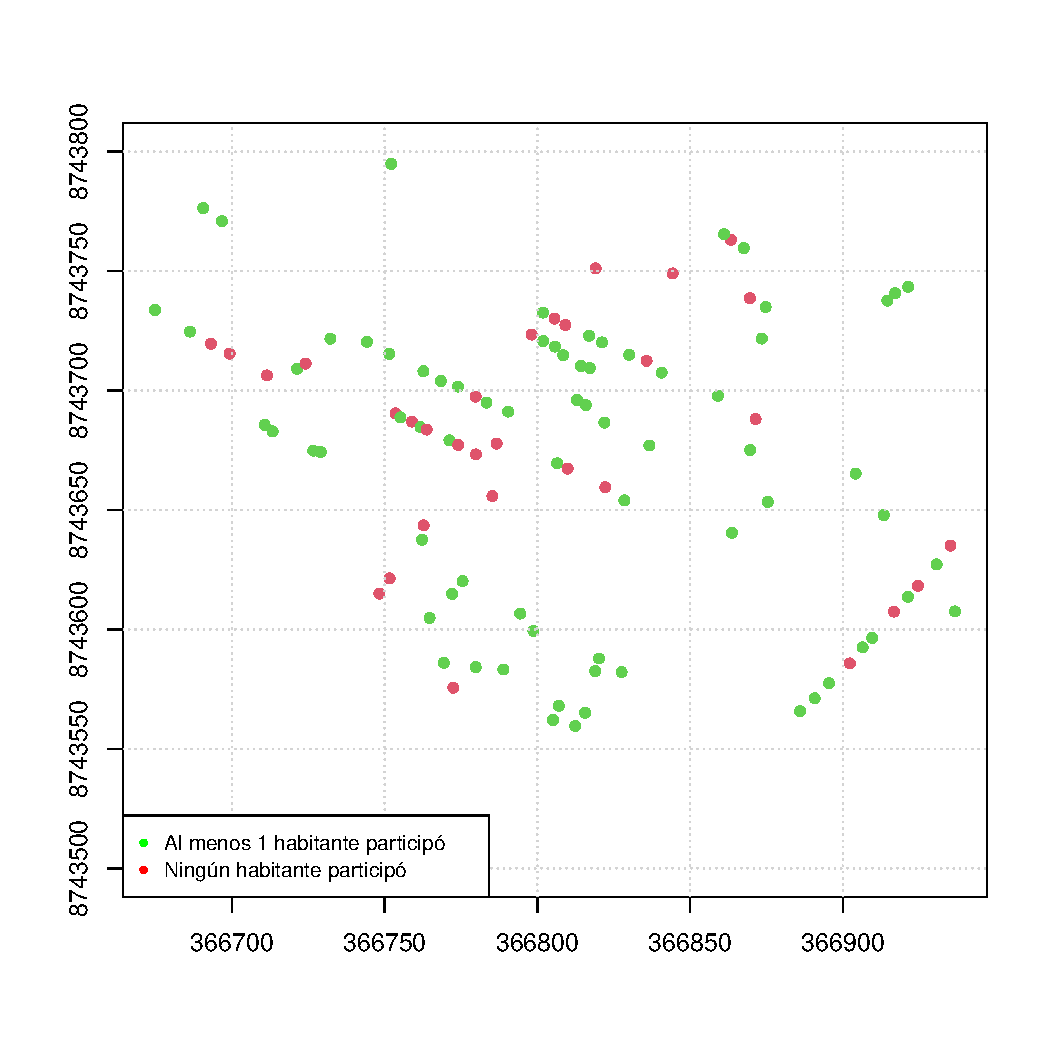
\includegraphics[width=0.85\textwidth]{graficos/houses_participation.pdf}
	\end{center}
	\caption{Distribución en el espacio de las casas habitadas en el centro poblado de Corpacancha.}
\end{figure}

\newpage

\begin{figure}[h]\label{houses_hidatidosis}
	\begin{center}
		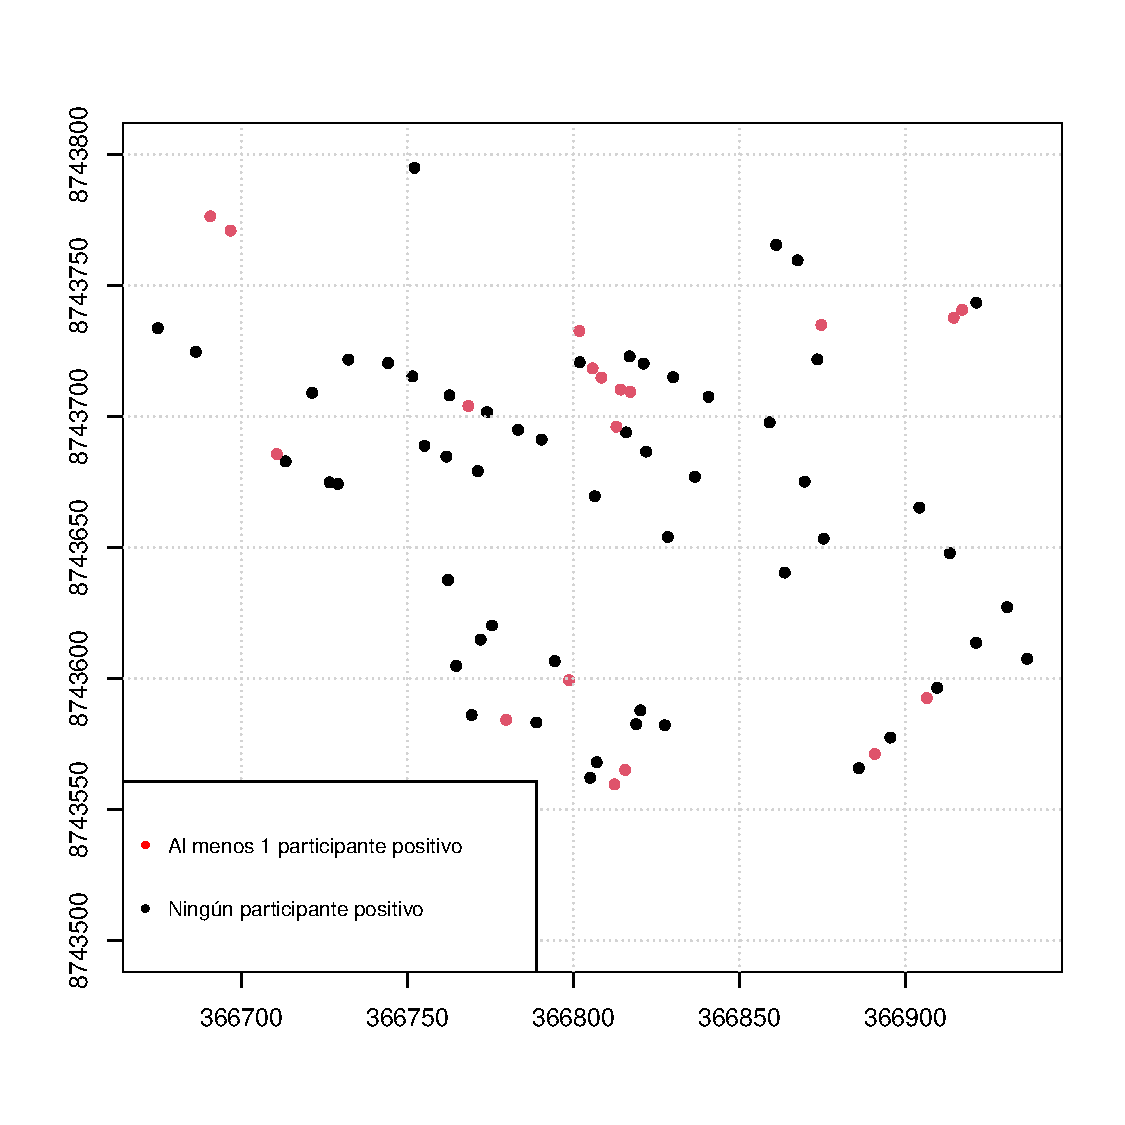
\includegraphics[width=0.85\textwidth]{graficos/houses_hidatidosis.pdf}
	\end{center}
	\caption{Distribución de las casas con al menos un habitante que haya participado en la campaña realizada en el centro poblado de Corpacancha.}
\end{figure}

\newpage

\begin{figure}[h]\label{prevalence_samplesize}
	\begin{center}
		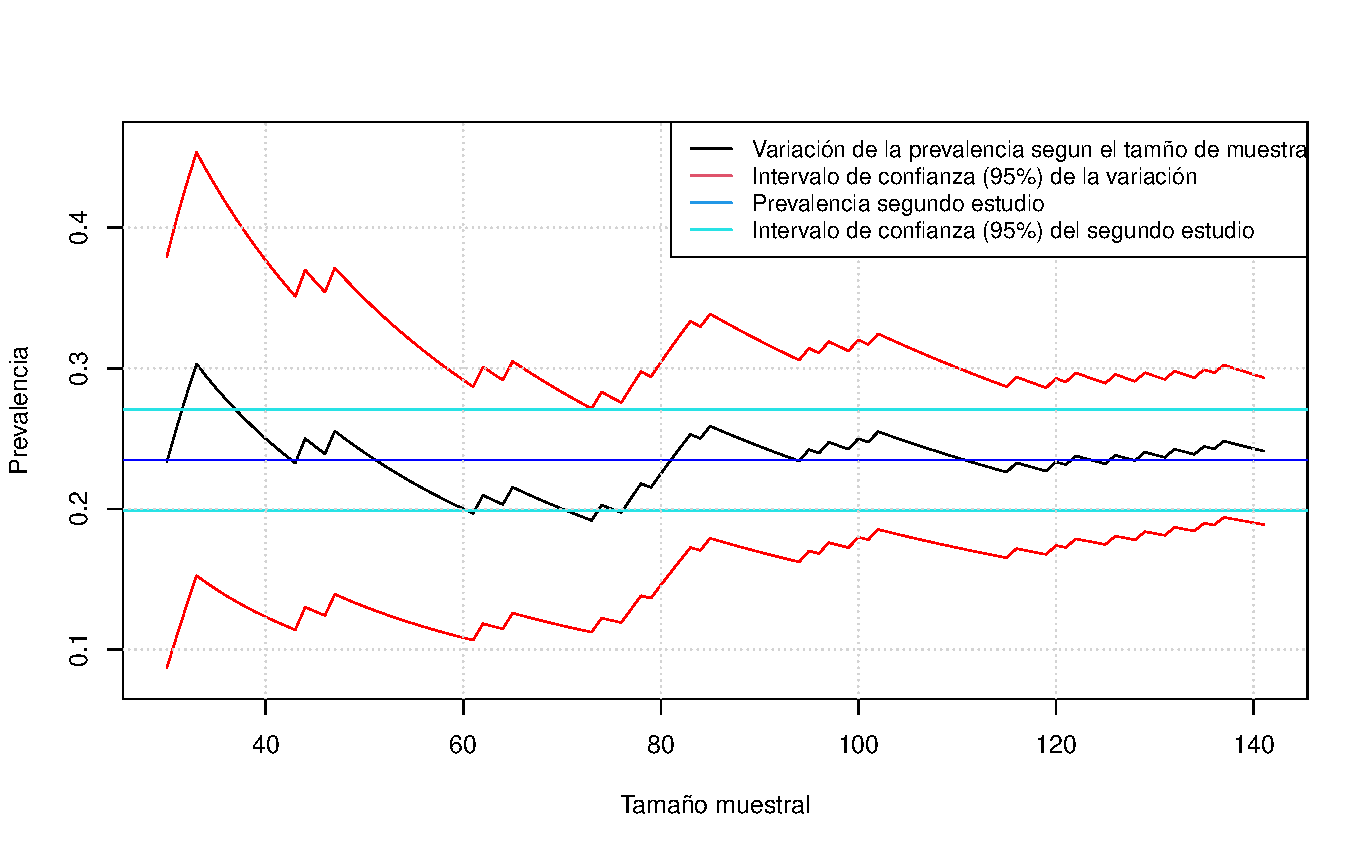
\includegraphics[width=1\textwidth]{graficos/prevalence_samplesize.pdf}
	\end{center}
	\caption{Prevalencia de Hidatidosis Humana en Corpacancha.}
\end{figure}

\newpage

\subsection{Análisis de los factores de riesgo}
De la base de datos, se seleccionaron como covariables a los factores de riesgo determinados en estudios anteriores en la región~\cite{santivanez2010factores}. El resumen de esta información, tanto univariado, como bivariado respecto a la prevalencia, se puede encontrar en las tablas \ref{DescripFactRiesPrev} y \ref{PrevFact}. En esta segunda tabla se observaron diferencias que fueron necesarias estudiar.

\begin{table}[h]
	\centering
	\caption{Factores de riesgo y prevalencia (n=141).}\label{DescripFactRiesPrev}
	\begin{tabular}{llll}
		\toprule
		\textbf{Características} &       & \multicolumn{1}{c}{\textbf{n}} & \multicolumn{1}{c}{\textbf{\%}} \\
		\midrule
		\multicolumn{2}{l}{Sexo} &       &  \\
		& Femenino & \multicolumn{1}{c}{83} & \multicolumn{1}{c}{58.9} \\
		& Masculino & \multicolumn{1}{c}{58} & \multicolumn{1}{c}{41.1} \\
		\midrule
		\multicolumn{2}{l}{Edad *} & \multicolumn{2}{c}{33.27 ($\pm$ 3.19)} \\
		\midrule
		\multicolumn{2}{l}{Nùmero de perros} &       &  \\
		& 0     & \multicolumn{1}{c}{95} & \multicolumn{1}{c}{67.4} \\
		& 1     & \multicolumn{1}{c}{15} & \multicolumn{1}{c}{10.6} \\
		& 2     & \multicolumn{1}{c}{17} & \multicolumn{1}{c}{12.1} \\
		& 3     & \multicolumn{1}{c}{11} & \multicolumn{1}{c}{7.8} \\
		& 4     & \multicolumn{1}{c}{3} & \multicolumn{1}{c}{2.1} \\
		\midrule
		\multicolumn{2}{l}{Prevalencia**} & \multicolumn{2}{c}{0.241 ($\pm$ 0.054)} \\
		\midrule
		\multicolumn{4}{l}{* Promedio (IC 95\%)} \\
		\multicolumn{4}{l}{** Proporción (IC 95\%)} \\
	\end{tabular}% 
\end{table}%

\newpage

\begin{table}[h]
	\centering
	\caption{Factores de riesgo por resultado de la campaña (n=141).}\label{PrevFact}
	\begin{tabular}{llll}
		\toprule
		\multicolumn{2}{l}{\textbf{Factor de riesgo}} & \multicolumn{1}{c}{\textbf{Positivo}} & \multicolumn{1}{c}{\textbf{Negativo}} \\
		\midrule
		\multicolumn{2}{l}{Sexo} &       &  \\
		& \multicolumn{1}{c}{Male} & \multicolumn{1}{c}{16 (27.6\%)} & \multicolumn{1}{c}{42 (72.4\%)} \\
		& \multicolumn{1}{c}{Female} & \multicolumn{1}{c}{18 (21.7\%)} & \multicolumn{1}{c}{65 (78.3\%)} \\
		\midrule
		\multicolumn{2}{l}{Edad*} & \multicolumn{1}{c}{36.1 $\pm$ 6.7} & \multicolumn{1}{c}{32.4 $\pm$ 3.6} \\
		\midrule
		\multicolumn{2}{l}{Número de perros} &       &  \\
		& \multicolumn{1}{c}{0} & \multicolumn{1}{c}{21 (22.1\%)} & \multicolumn{1}{c}{74 (77.9\%)} \\
		& \multicolumn{1}{c}{1} & \multicolumn{1}{c}{2 (13.3\%)} & \multicolumn{1}{c}{13 (86.7\%)} \\
		& \multicolumn{1}{c}{2} & \multicolumn{1}{c}{3 (17.6\%)} & \multicolumn{1}{c}{14 (82.4\%)} \\
		& \multicolumn{1}{c}{3} & \multicolumn{1}{c}{7 (63.6\%)} & \multicolumn{1}{c}{4 (36.4\%)} \\
		& \multicolumn{1}{c}{4} & \multicolumn{1}{c}{1 (33.3\%)} & \multicolumn{1}{c}{2 (66.7\%)} \\
		\midrule
		\multicolumn{4}{l}{* Media por resultado} \\
	\end{tabular}%
\end{table}%


\subsubsection{Sexo}
En la tabla \ref{PrevFact}, se observó que hay una diferencia en la prevalencia por sexo de la persona. Pese a esto, la diferencia encontrada no era significativa debido a la superposición de los invervalos de confianza de cada una (Fig. \ref{bar_sexoprevalencia}).

\begin{figure}[h]
	\centering
	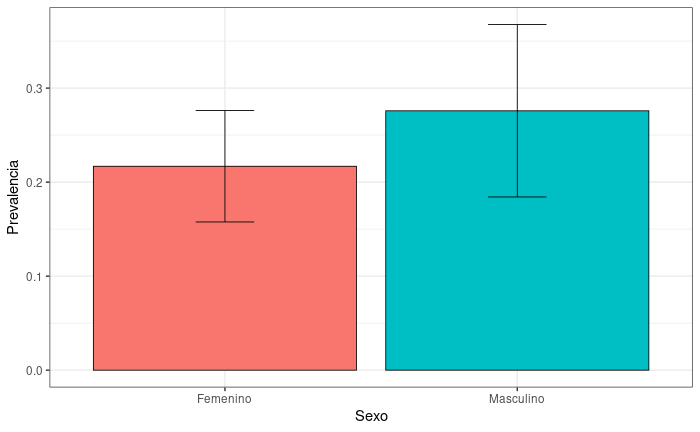
\includegraphics[width=0.7\textwidth]{graficos/sexoprevalencia.png}
	\caption{Prevalencia e intervalo de confianza por sexo.}
	\label{bar_sexoprevalencia}
\end{figure}

\newpage

Ajustando un modelo lineal generalizado entre el sexo y la prevalencia de hidatidosis, se observó que la posibilidad de tener hidatidosis siendo hombre es 1.38 veces la posibilidad siendo mujer (Tabla \ref{or_sexo}). Pese a que los resultados no son significativos, esto no descarta que se considere como factor de riesgo debido a que el p-valor se encuentra relacionado con la potencia estadística que tuvo la muestra~\cite{ellis2010essential}.


\begin{table}[h]
	\centering
	\caption{Odd Ratio de la variable sexo}
	\label{or_sexo}
	\begin{tabular}{lccc}
		\hline
		& OR*   & IC 95\%           & p-valor \\ \hline
		\multicolumn{1}{c}{Sexo = Masculino}  & 1.38  & [0.63; 3.00] & 0.421   \\ \hline
		\multicolumn{4}{l}{*obtenido al ajustar un modelo lineal generalizado}
	\end{tabular}
\end{table}

\subsubsection{Edad}
En la tabla \ref{PrevFact}, se observó que hay una diferencia en la edad promedio entre el grupo positivo a la enfermedad y el grupo negativo a la enfermedad. No obstante, esta diferencia resultó ser no significativa pues sus intervalor de confianza se superponen. Ajustando un modelo lineal generalizado entre el edad y la prevalencia de hidatidosis, se observó que la posibilidad de tener hidatidosis se incrementaba 1.01 veces con cada año de edad (Tabla \ref{or_edad}). Pese a que los resultados no son significativos, esto no descarta que se considere como factor de riesgo. Esto debido a que el p-valor se encuentra relacionado con la potencia estadística que tuvo la muestra~\cite{ellis2010essential}.

\begin{table}[h]
	\centering
	\caption{Odd Ratio de la variable edad}
	\label{or_edad}
	\begin{tabular}{lccc}
		\hline
		& OR*   & IC 95\%          & p-valor \\ \hline
		\multicolumn{1}{c}{Edad}  & 1.01  & [0.99; 1.03] & 0.334   \\ \hline
		\multicolumn{4}{l}{*obtenido al ajustar un modelo lineal generalizado}
	\end{tabular}
\end{table}

\newpage

\subsubsection{Número de perros}
En la tabla \ref{PrevFact}, se observó que hay una diferencia en la prevalencia por el número de perros que se tienen. La diferencia encontrada era significativa cuando se dicotomizaba la variable del número de perros. Esto debido a la no superposición de los invervalos de confianza de cada una (Fig. \ref{fig:bar_perrosprevalencia}). Ajustando un modelo lineal generalizado entre el número de perros y la prevalencia de hidatidosis, se observó que la posibilidad de tener hidatidosis teniendo menos de tres perros es 0.19 veces la posibilidad teniendo al menos tres perros (Tabla \ref{or_sexo}). Esto determinó que en adeltante, la variable número de perros sea tomada como cualitativa con dos categoría: menos de tres perros y al menos tres perros.

\begin{figure}[h]
	\centering
	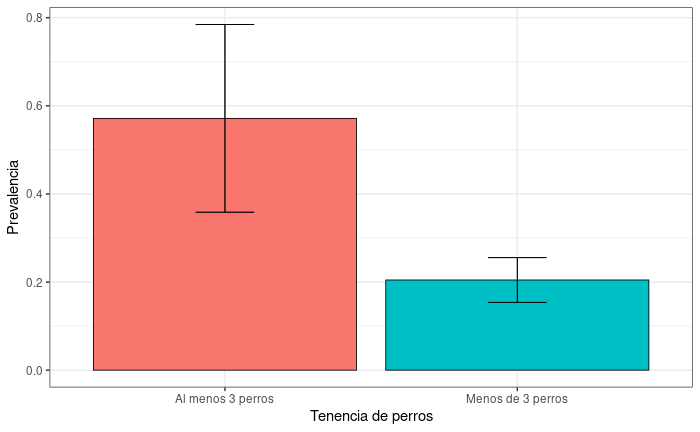
\includegraphics[width=0.7\textwidth]{graficos/perrosprevalencia.png}
	\caption{Prevalencia e intervalo de confianza por tenencia de perros.}
	\label{fig:bar_perrosprevalencia}
\end{figure}

\begin{table}[h]
	\centering
	\caption{Odd Ratio de la variable perro}
	\label{or_perros}
	\begin{tabular}{cccc}
		\hline
		\multicolumn{1}{l}{}          & OR*     & IC 95\%              & p-valor   \\ \hline
		Perros = 1                    & 0.54    & [0.08; 2.17]     & 0.443     \\
		Perros = 2                    & 0.76    & [0.16; 2.59]     & 0.681     \\
		Perros = 3                    & 6.17    & [1.70; 25.49]    & 0.007     \\
		Perros = 4                    & 1.76    & [0.08; 19.28]    & 0.650     \\ \hline
		Perros = Menos de 3 perros    & 0.19    & [0.06; 0.60]     & 0.005     \\ \hline
		\multicolumn{4}{l}{*obtenido al ajustar un modelo lineal generalizado}
	\end{tabular}
\end{table}

\newpage
\subsection{Análisis de la intensidad}
Se observó que la población se concentra al sureste del centro de salud en el que se hizo la campaña (Fig. \ref{intensity_population}). Se encontró un comportamiento similar en los habitantes que participaron en la campaña (Fig. \ref{intensity_sample}). No obstante, era necesario observar si la razón de las intensidades se mantiene constante en el espacio. En la figura \ref{risk_to_sampling} se observó que el riesgo de participar en la muestra no es constante en el área; especialmente en la zona noroeste. Esto planteó la existencia  de un posible sesgo espacial.

\begin{figure}[h]
	\centering
	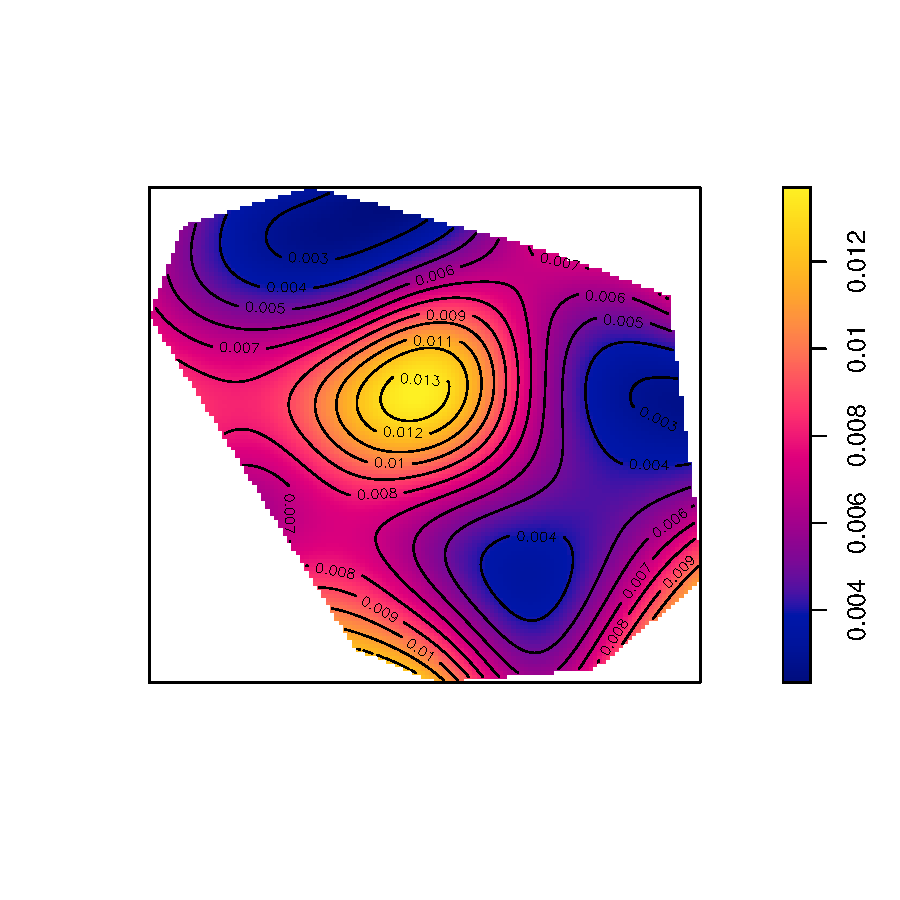
\includegraphics[width=0.9\textwidth]{graficos/intensity_population.pdf}
	\caption{Intensidad poblacional} \label{intensity_population}
\end{figure}

\newpage

\begin{figure}[h]
	\centering
	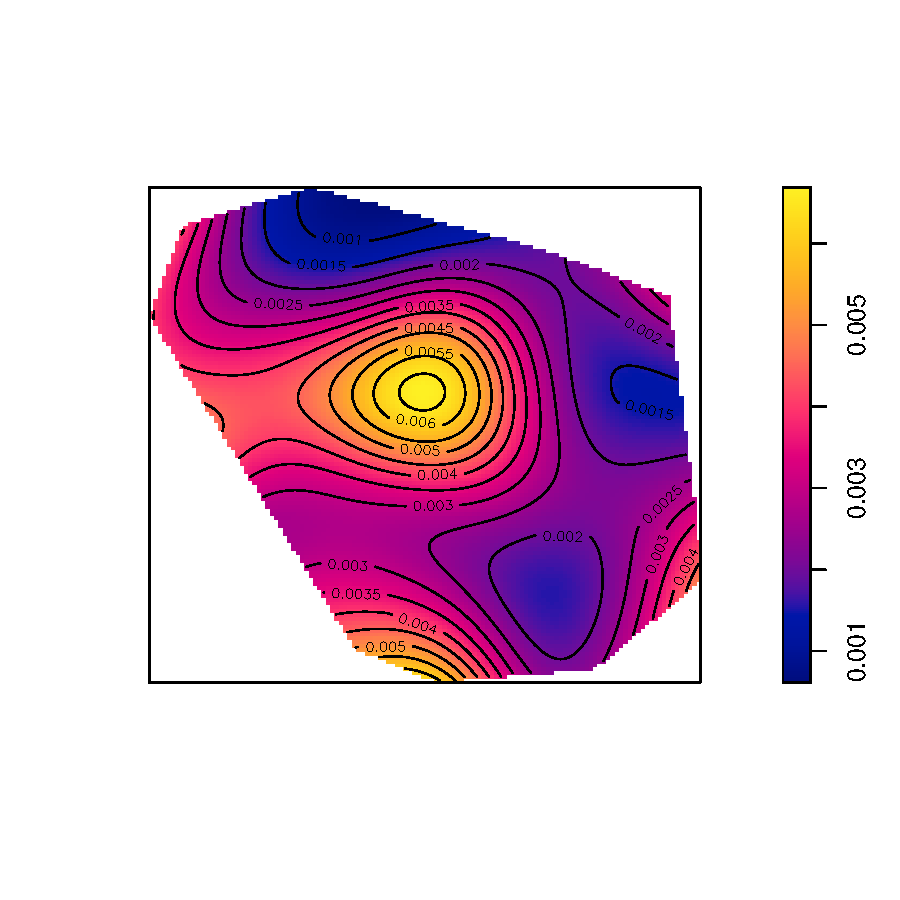
\includegraphics[width=0.9\textwidth]{graficos/intensity_sample.pdf}
	\caption{Intensidad muestral} \label{intensity_sample}
\end{figure}

\newpage

\begin{figure}[h]
	\centering
	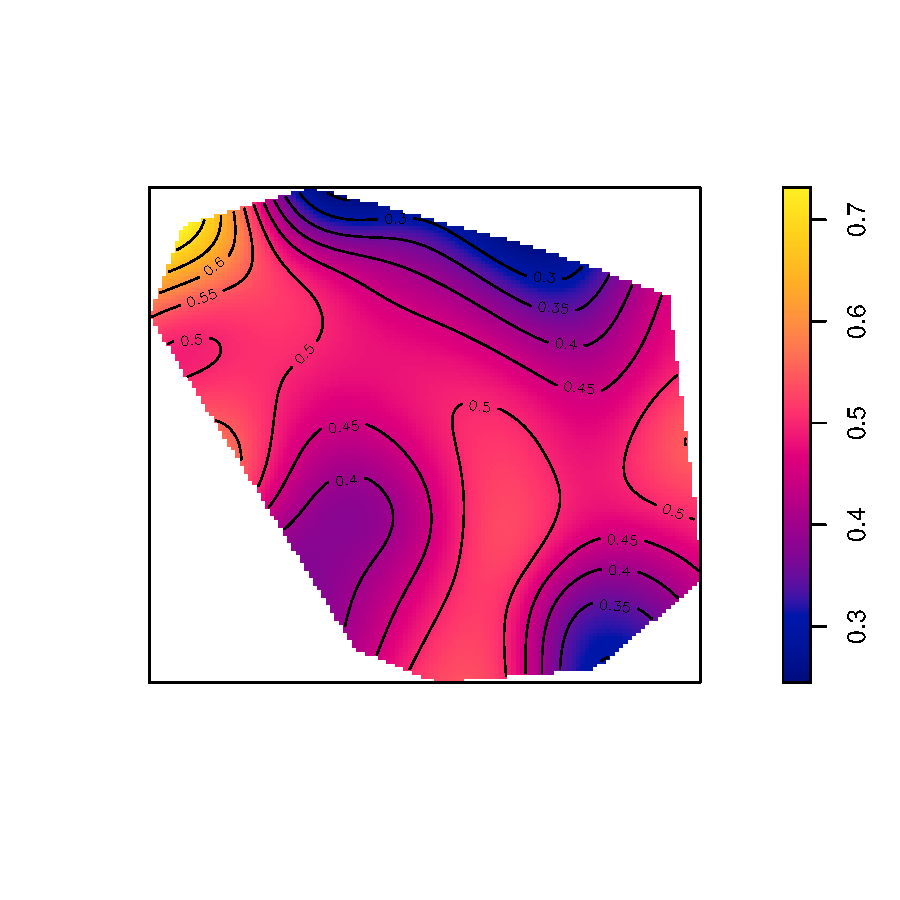
\includegraphics[width=0.9\textwidth]{graficos/risk_to_sampling.pdf}
	\caption{Riesgo de participar en la muestra}
	\label{risk_to_sampling}
\end{figure}

\newpage

Lo visto en la Figura \ref{risk_to_sampling} indicó la necesidad de corregir el riesgo de tener la enfermedad a nivel espacial (Fig.~\ref{risk_to_disease}).
\begin{figure}[h]
	\centering
	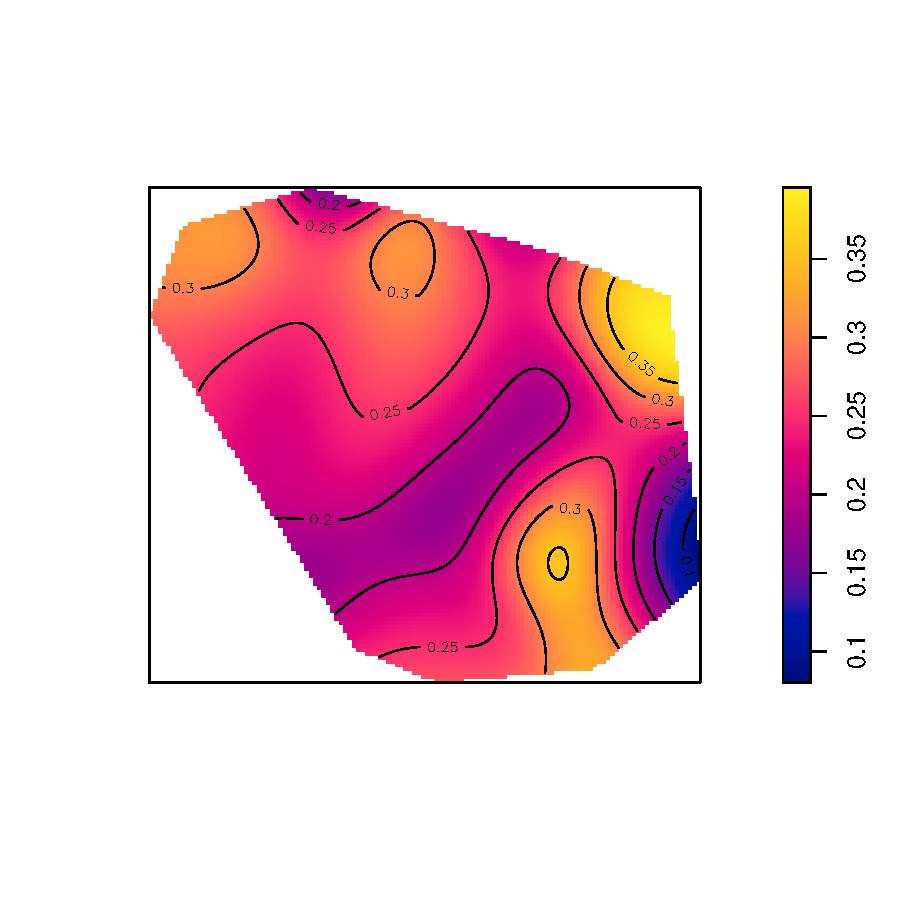
\includegraphics[width=0.9\textwidth]{graficos/risk_to_disease.pdf}
	\caption{Riesgo de tener la enfermedad}
	\label{risk_to_disease}
\end{figure}

\newpage

\section{Simulaciones}

Cada una de las simulaciones y sus resultados fueron evaluados por escenario (Tabla \ref{simu_resul}, Figura \ref{simu_01-09} y Figura \ref{simu_10-18}). Si bien el ECM($\tilde{\theta}$) resultó ser mayor al ECM($\hat{\theta}$) en cada escenario, también se observó que en su mayoría estos superaron el 15\% de éxito; o sea, que en 13 de 18 escenarios, al menos el 15\% de las simulaciones, la estimación de la prevalencia por medio del método presentado tenía un valor más cercano al real que la estimación por el método convencional. Este comportamiento también se observó en los escenarios con las caraterísticas más similares a la data real, a nivel de cobertura y tamaño poblacional. Pese a esto, las curvas de densidad en cada escenario presentaron notorias diferencias entre si.


\begin{table}[h]
	\centering
	\caption{Resultados de la simulación}
	\label{simu_resul}
	\begin{tabular}{cccccccc}
		\hline
		Escenario & m   & Éxitos (\%) & $\hat{n}$ & Cobertura & Prevalencia* & ECM($\hat{\theta}$) & ECM($\tilde{\theta}$) \\ \hline
		1         & 506 & 33.20      & 249        & 34.67     & 0.252       & 0.0014 & 0.0037 \\
		2         & 510 & 23.92      & 249        & 44.95     & 0.250       & 0.0009 & 0.0049 \\
		3         & 509 & 21.61      & 250        & 54.86     & 0.251       & 0.0006 & 0.0053 \\
		4         & 510 & 23.53      & 349        & 35.09     & 0.251       & 0.0010 & 0.0066 \\
		5         & 510 & 15.69      & 350        & 44.94     & 0.249       & 0.0007 & 0.0080 \\
		6         & 510 & 10.78      & 350        & 54.86     & 0.252       & 0.0004 & 0.0087 \\
		7         & 510 & 14.12      & 451        & 35.09     & 0.249       & 0.0007 & 0.0118 \\
		8         & 510 & 8.43       & 450        & 45.08     & 0.251       & 0.0005 & 0.0108 \\
		9         & 510 & 6.47       & 450        & 55.21     & 0.251       & 0.0003 & 0.0098 \\
		10        & 509 & 15.52      & 247        & 34.28     & 0.241       & 0.0040 & 0.0271 \\
		11        & 499 & 15.83      & 246        & 44.38     & 0.243       & 0.0009 & 0.0153 \\
		12        & 510 & 16.86      & 247        & 55.41     & 0.242       & 0.0007 & 0.0088 \\
		13        & 503 & 20.68      & 344        & 34.50     & 0.242       & 0.0033 & 0.0259 \\
		14        & 506 & 16.60      & 342        & 44.20     & 0.243       & 0.0007 & 0.0127 \\
		15        & 509 & 15.52      & 343        & 55.47     & 0.243       & 0.0005 & 0.0080 \\
		16        & 510 & 21.96      & 440        & 34.40     & 0.241       & 0.0034 & 0.0236 \\
		17        & 510 & 15.69      & 440        & 44.16     & 0.242       & 0.0005 & 0.0124 \\
		18        & 510 & 14.51      & 440        & 55.36     & 0.242       & 0.0004 & 0.0088 \\ \hline
		\multicolumn{8}{l}{m: Número de simulaciones por escenario}                           \\
		\multicolumn{8}{l}{n: Número promedio de personas por escenario}                      \\
		\multicolumn{8}{l}{Cobertura*: Cobertura de muestreo promedio por escenario}          \\
		\multicolumn{8}{l}{Prevalencia*: Prevalencia promedio por escenario}                  \\ \hline
	\end{tabular}
\end{table}

\newpage

\begin{figure}[h] 
	\centering
	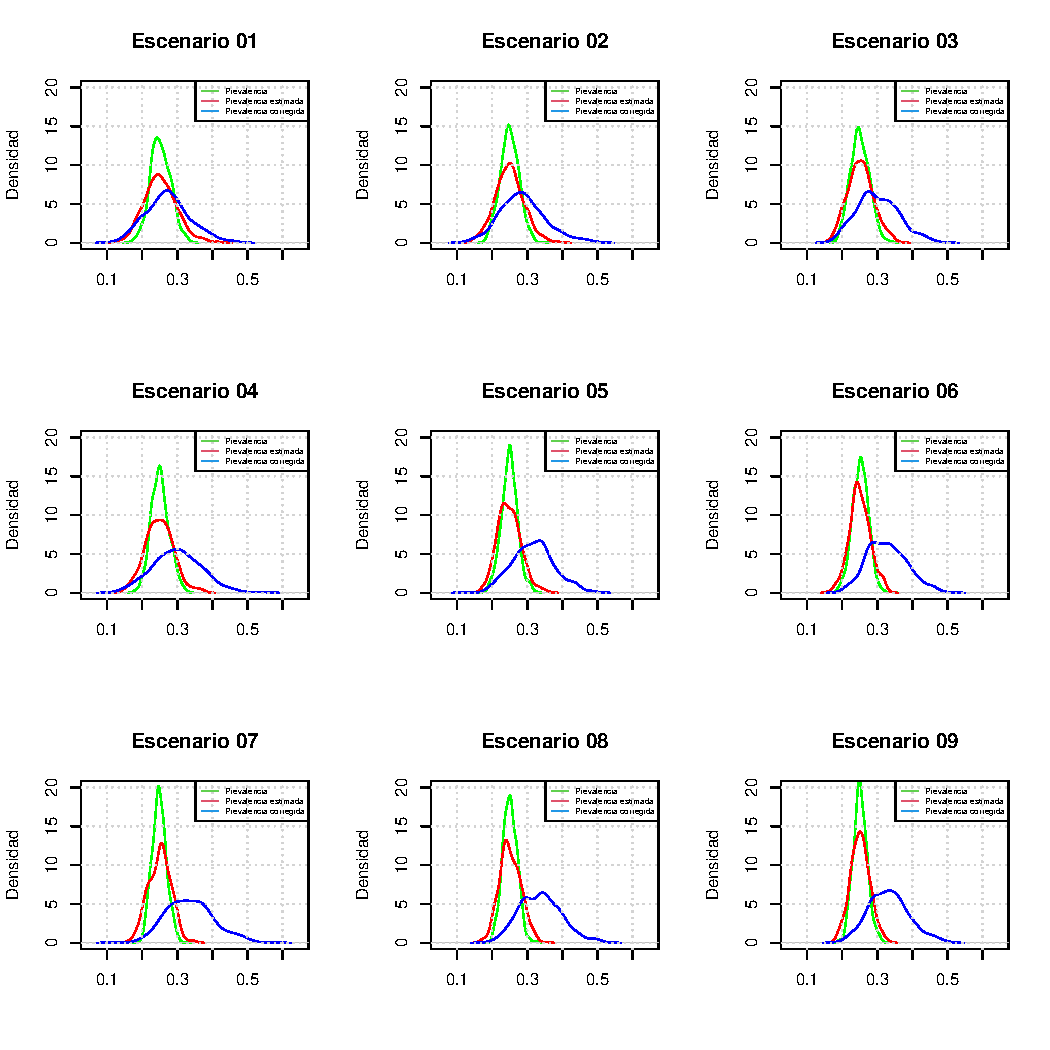
\includegraphics[width=1\textwidth]{graficos/simu_01-09.pdf}
	\caption{Densidad del parámetro de los escenarios 1 al 9} \label{simu_01-09}
\end{figure}

\newpage

\begin{figure}[h] 
	\centering
	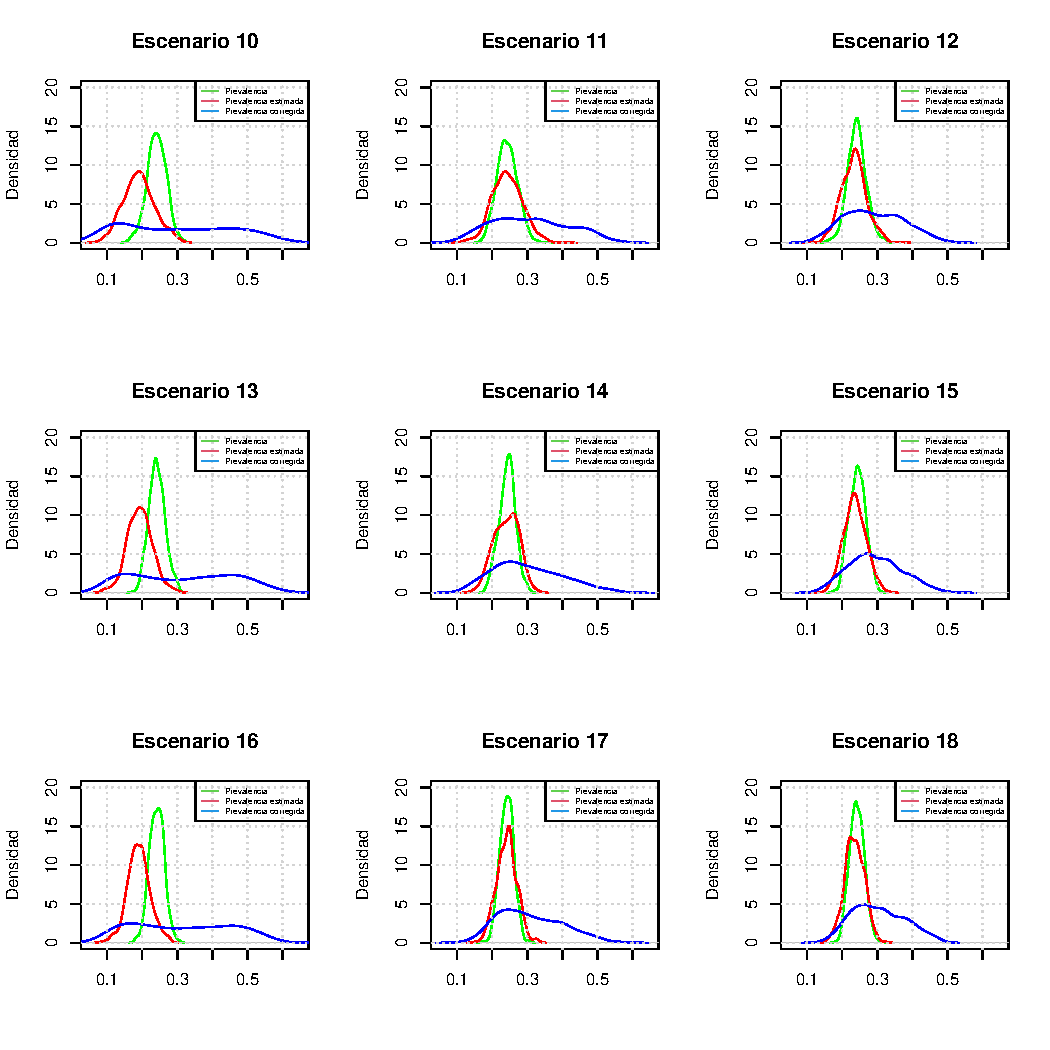
\includegraphics[width=1\textwidth]{graficos/simu_10-18.pdf}
	\caption{Densidad del parámetro de los escenarios 10 al 18} \label{simu_10-18}
\end{figure}


\newpage

\section{Modelamiento}
\subsection{Intensidad}
\label{seccion_intensidad}
En la estimación de la función de intensidad para la población y la muestra, los modelos se ajustaron con 14 y 16 funciones de base, respectivamente, en base a sus residuales (Véase Fig.~\ref{intensity_population_residuals} y~\ref{intensity_sample_residuals} )

\subsubsection{Homogeneidad de riesgo}

En base al algoritmo \ref{validaHipo}, se determinó que el riesgo al ser seleccionado es no homogéneo, debido a que en más de una observación, el cociente entre las dos intensidades no se ha encontrado en el intervalo de confianza correspondiente. Este resultado confirmó lo visto en la Figura \ref{risk_to_sampling}.

%\begin{figure}[h] 
%	\centering
%	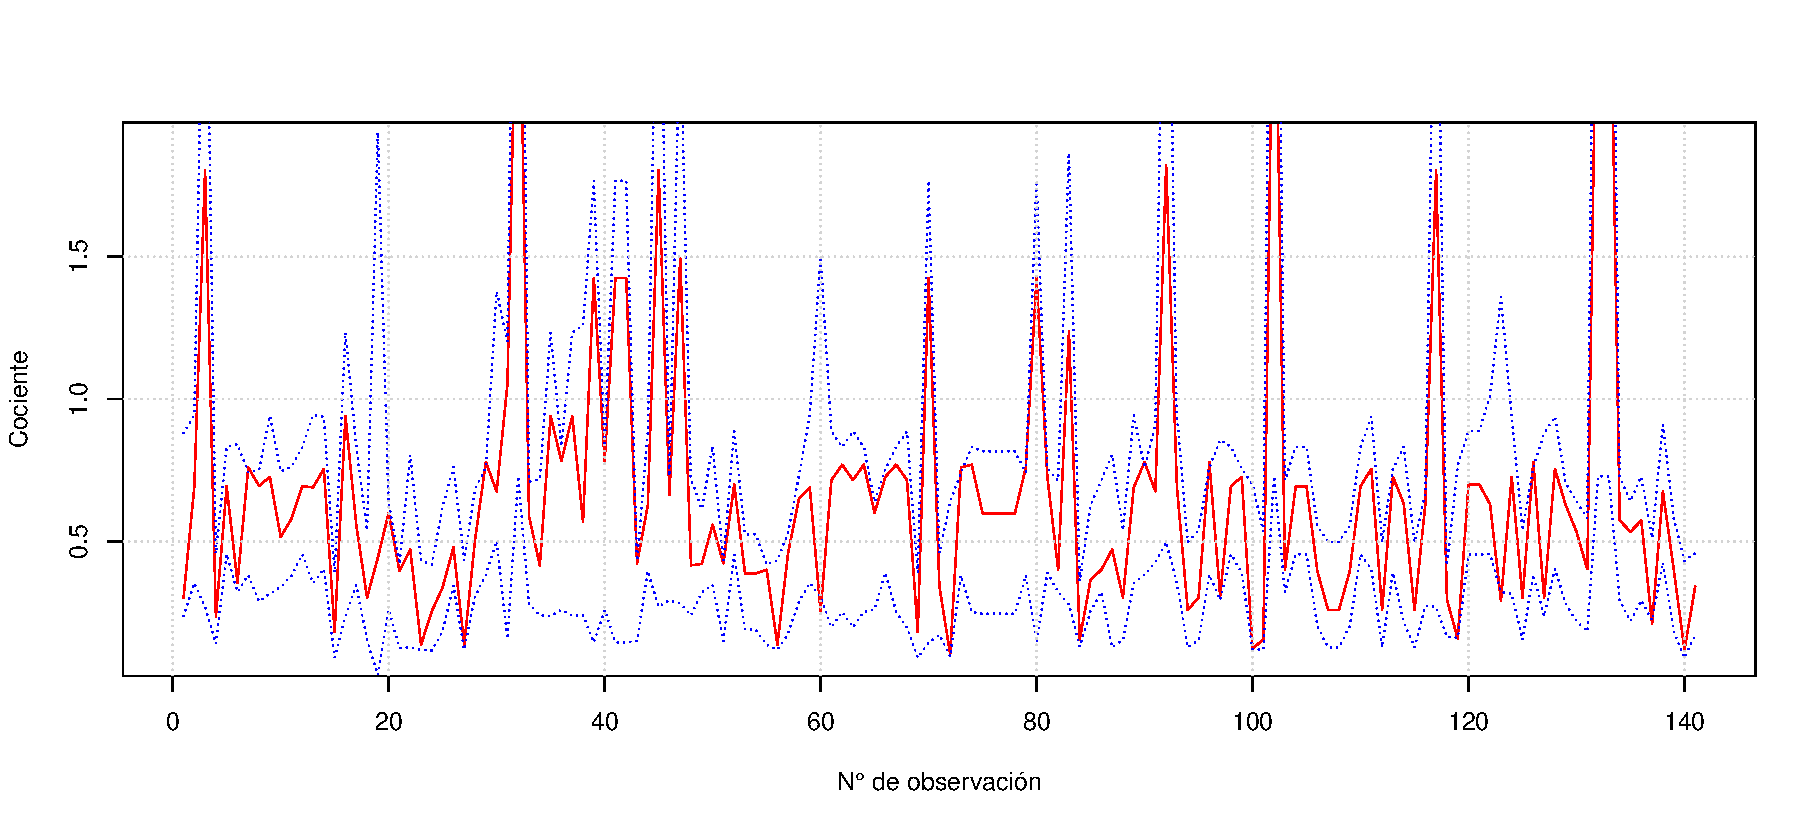
\includegraphics[width=1\textwidth]{graficos/montecarlo.pdf}
%	\caption{Cociente de intensidades} \label{montecarlo}
%\end{figure}


\newpage

\begin{figure}[h] 
	\centering
	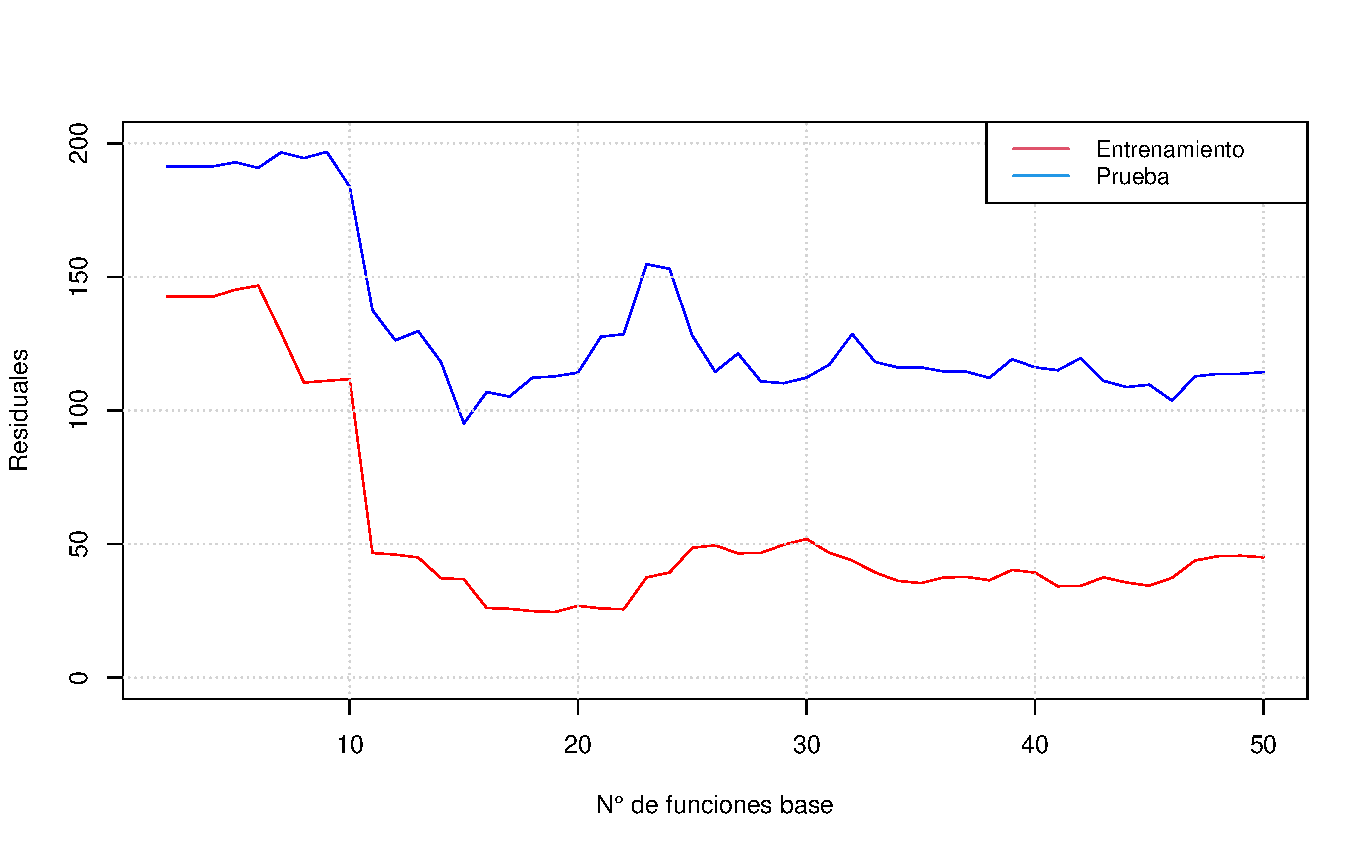
\includegraphics[width=0.67\textwidth]{graficos/intensity_population_residuals.pdf}
	\caption{Residuales en la población} \label{intensity_population_residuals}
\end{figure}

\begin{figure}[h]
	\centering
	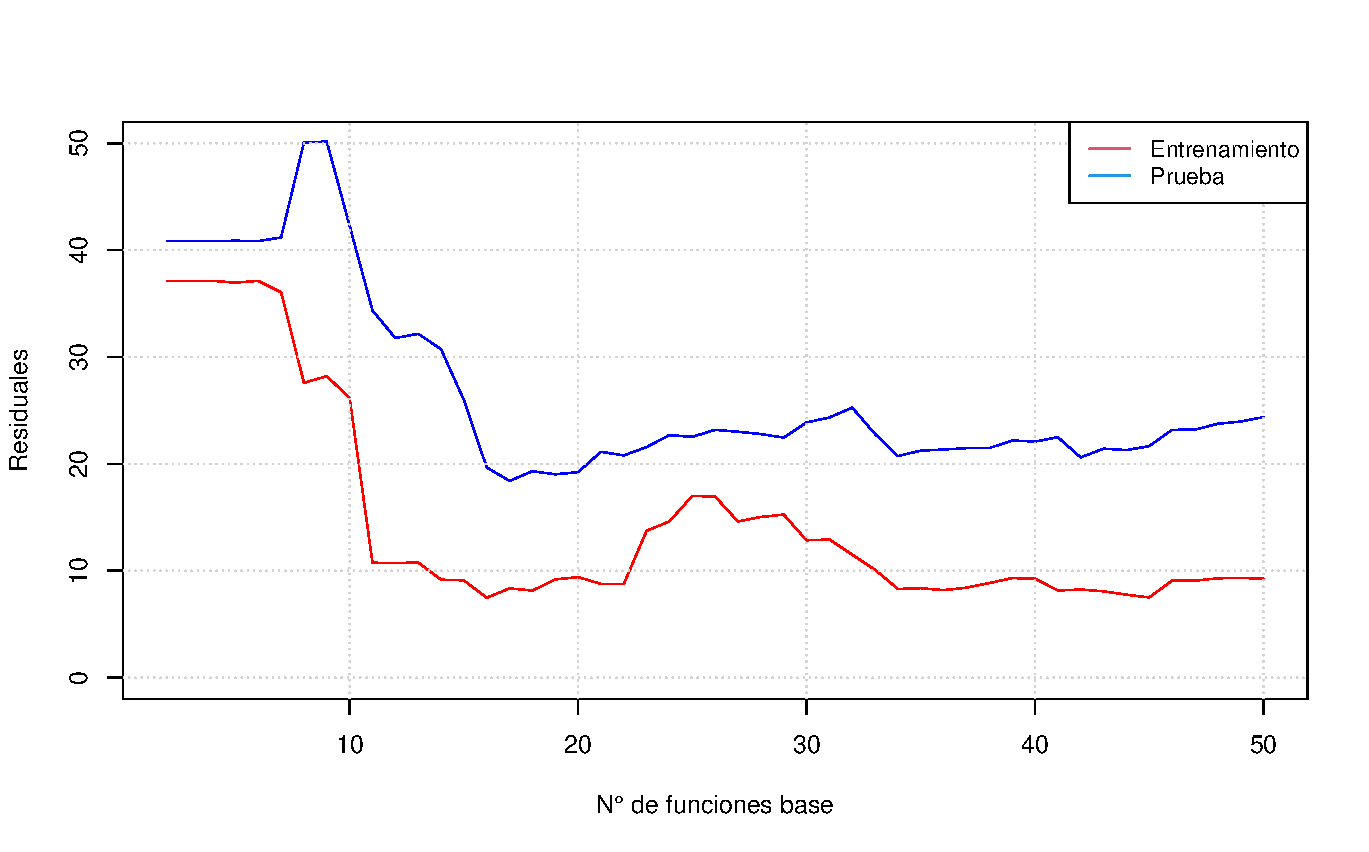
\includegraphics[width=0.67\textwidth]{graficos/intensity_sample_residuals.pdf}
	\caption{Residuales en la muestra} \label{intensity_sample_residuals}
\end{figure}

\newpage


\subsection{Riesgo}
Comparando las métricas de ajuste del grupo de entrenamiento y del grupo de prueba de cada modelo ajustado (Tabla~\ref{model_metricas}), se encontró una mejora en los modelos al introduccir el factor de corrección w, salvo aquel modelo que solo consideró el efecto espacial de las observaciones (Modelo espacial). Este mismo comportamiento se observó cuando a las covariables comprendidas como factores de riesgo (edad, sexo, tener al menos 3 perros) se les añadió la variable del efecto espacial. En base a estos resultados, se seleccionó al \textit{Modelo completo (w)}, compuesto por los factores de riesgo, el efecto espacial y el factor de correción w, como el modelo más adecuado para la inferencia y estimación del valor de la prevalencia corregida.

% Please add the following required packages to your document preamble:
% \usepackage{booktabs}
% \usepackage{multirow}
\begin{center}
	\begin{table}[h]
		\centering
		\caption{Métricas de ajuste para los modelos}
		\label{model_metricas}
		\begin{tabular}{@{}lcccccc@{}}
			\toprule
			\multicolumn{1}{c}{\multirow{2}{*}{Modelo}} & \multicolumn{3}{c}{Entrenamiento}                          & \multicolumn{3}{c}{Prueba}            \\ \cmidrule(l){2-7} 
			\multicolumn{1}{c}{}                        & Esp. & Sens. & \multicolumn{1}{c|}{AUC}    & Esp. & Sens. & AUC    \\ \midrule
			\multicolumn{1}{l|}{Modelo espacial}            & 1             & 0       & \multicolumn{1}{c|}{0.5381} & -       & -            & 0.6766 \\
			\multicolumn{1}{l|}{Modelo espacial (w)}            & 0.96             & 0.125       & \multicolumn{1}{c|}{0.5864} & -       & -            & 0.5453 \\
			\multicolumn{1}{l|}{Modelo edad}            & 1             & 0.0833       & \multicolumn{1}{c|}{0.5578} & 0.03125       & 1            & 0.5672 \\
			\multicolumn{1}{l|}{Modelo edad (w)}        & 0.9333        & 0.2917       & \multicolumn{1}{c|}{0.6122} & 0.59375       & 0.6          & 0.6453 \\
			\multicolumn{1}{l|}{Modelo sexo}            & 1             & 0            & \multicolumn{1}{c|}{0.5358} & 1             & 0            & 0.5469 \\
			\multicolumn{1}{l|}{Modelo sexo (w)}        & 1             & 0            & \multicolumn{1}{c|}{0.4642} & 1             & 0            & 0.5469 \\
			\multicolumn{1}{l|}{Modelo perros}          & 0.9333        & 0.3333       & \multicolumn{1}{c|}{0.6333} & 0.9688        & 0            & 0.149  \\
			\multicolumn{1}{l|}{Modelo perros (w)}      & 0.9333        & 0.3333       & \multicolumn{1}{c|}{0.6333} & 0.9688        & 0            & 0.149  \\
			\multicolumn{1}{l|}{Modelo sexo edad}       & 1             & 0.0833       & \multicolumn{1}{c|}{0.6369} & 0.03125       & 1            & 0.5406 \\
			\multicolumn{1}{l|}{Modelo sexo edad (w)}   & 0.9467        & 0.4583       & \multicolumn{1}{c|}{0.8708} & 0.5625        & 0.8          & 0.7562 \\
			\multicolumn{1}{l|}{Modelo s. e. p.}        & 0.96          & 0.375        & \multicolumn{1}{c|}{0.74}   & 0.0938        & 0.9          & 0.5141 \\
			\multicolumn{1}{l|}{Modeso s. e. p. (w)}    & 0.9467        & 0.4583       & \multicolumn{1}{c|}{0.7144} & 0.625         & 0.5          & 0.5328 \\
			\multicolumn{1}{l|}{Modelo completo}        & 0.96          & 0.333        & \multicolumn{1}{c|}{0.7403} & 0.53125       & 0.5          & 0.6    \\
			\multicolumn{1}{l|}{Modelo completo (w)}    & 0.9733        & 0.375        & \multicolumn{1}{c|}{0.7503} & 0.5625        & 0.8          & 0.7438 \\ \bottomrule
		\end{tabular}
	\end{table}
	
\end{center}

\newpage

\section{Infererencia}

El modelo final, \textit{modelo completo (w)}, fue utilizado para inferir la presencia de la enfermedad en los datos no muestreados. Con esto se pudo estimar una prevalencia corregida del 0.22. Este valor, si bien se encontraba dentro del intervalo de confianza para el primer estudio, estaba por debajo de su valor puntual (0.241), comportamiento que se ha visto repetido en el segundo estudio (0.235). Esto indicó la presencia de una sobrestimación en la prevalencia del primer estudio.


\begin{figure}[h]
	\centering
	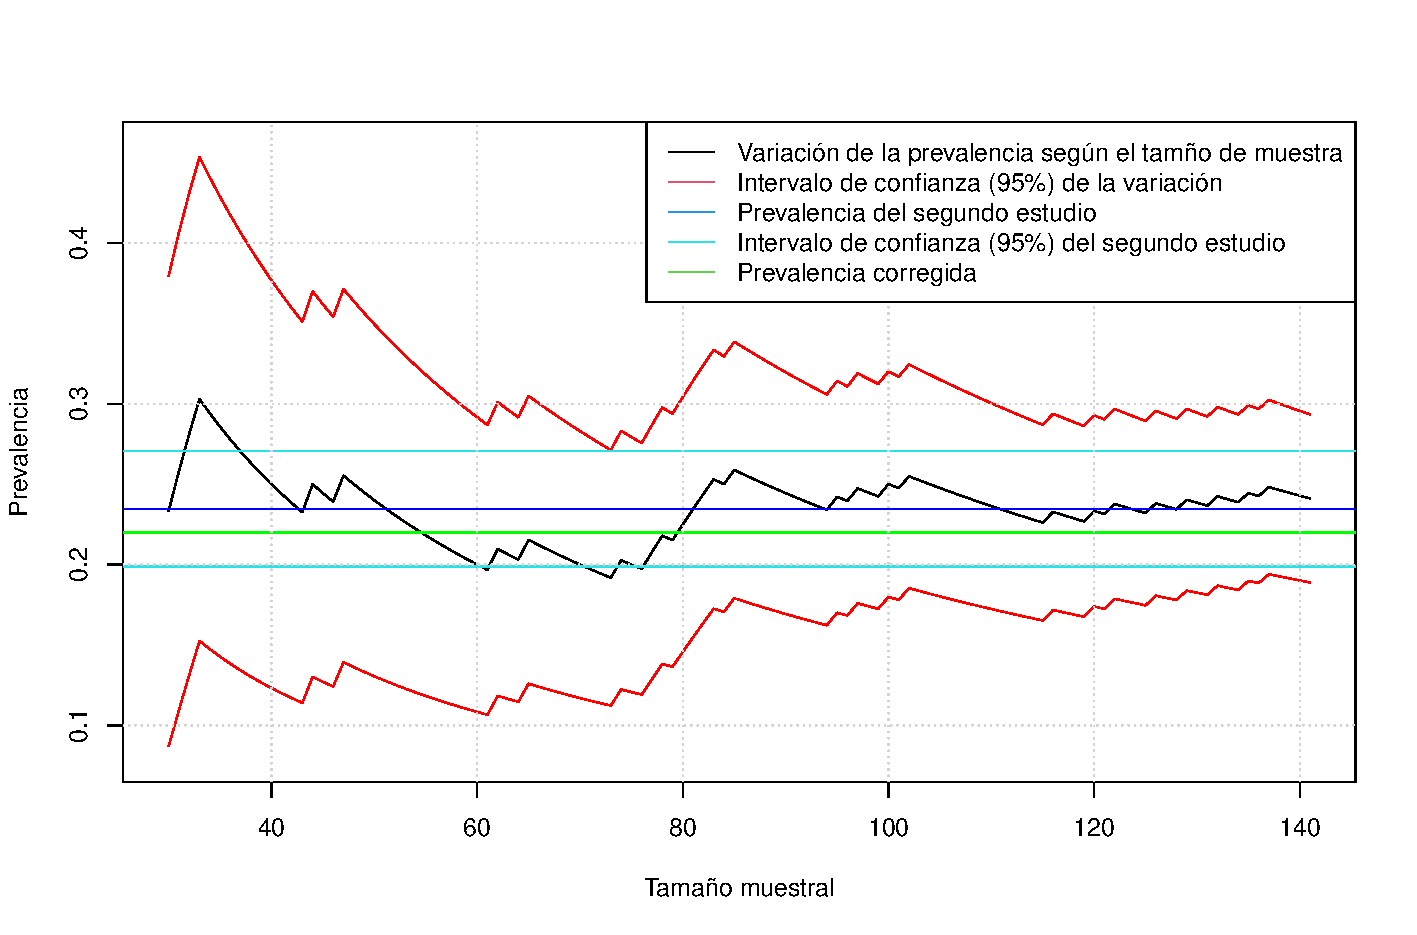
\includegraphics[width=1\textwidth]{graficos/prevalence_samplesize_fixed.pdf}
	\caption{Prevalencia de Hidatidosis Humana en Corpacancha, añadiendo la prevalencia corregida.}
	\label{prevalence_samplesize_fixed}
\end{figure}

\newpage
Esto permitió estimar un factor de corrección para la intesidad de $\rho$ = 1.126 (Véase~\ref{rho}). Empleando esto en~\ref{intesidad_rho}, se observó el cambio en el riesgo corregido de tener la enfermedad a nivel espacial en la población (Figura \ref{risk_to_disease_fixed}).
\begin{equation*}
	\hat{p}(x,y) = \cfrac{\hat{\lambda}_1(x,y)}{\hat{\lambda}_1(x,y)+ \rho \hat{\lambda}_0(x,y)} = \cfrac{\hat{\lambda}_1(x,y)}{\hat{\lambda}_1(x,y)+ 1.126* \hat{\lambda}_0(x,y)}
\end{equation*}

\begin{figure}[h]
	\centering
	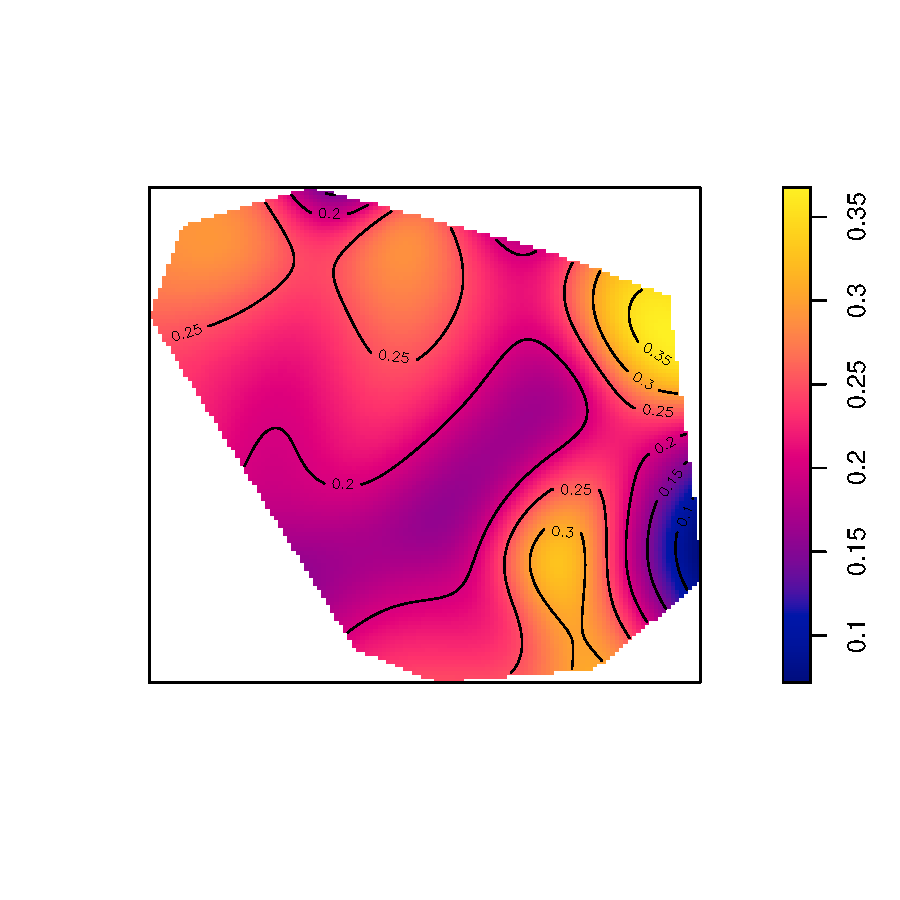
\includegraphics[width=0.9\textwidth]{graficos/risk_to_disease_fixed.pdf}
	\caption{Riesgo corregido de tener la enfermedad} \label{risk_to_disease_fixed}
\end{figure}




\newpage


\section{Implementación}
Con el fin de analizar la utilidad del método propuesto pero en otros contextos, se aplicó en el centro poblado de Canchayllo y se tuvo como resultado una prevalencia del $0.150$ ( $\pm 0.049$ IC$_{95\%}$  ).

\subsection*{Ajuste de intensidad}
Se ajustaron las intensidades correspondientes para la población y la muestra. El cociente de estas intensidades se puede ver en la Figura \ref{canchayllo_risk_to_sampling}, tal como en la sección \ref{seccion_intensidad}. La no homoegeniedad observada en esta figura se confirmó tras hacer la evaluación en base al algoritmo \ref{validaHipo}, debido a que en más de una observación, el cociente entre las dos intensidades no se ha encontrado en el intervalo de confianza correspondiente de acuerdo al algoritmo.


\begin{figure}[h]
	\centering
	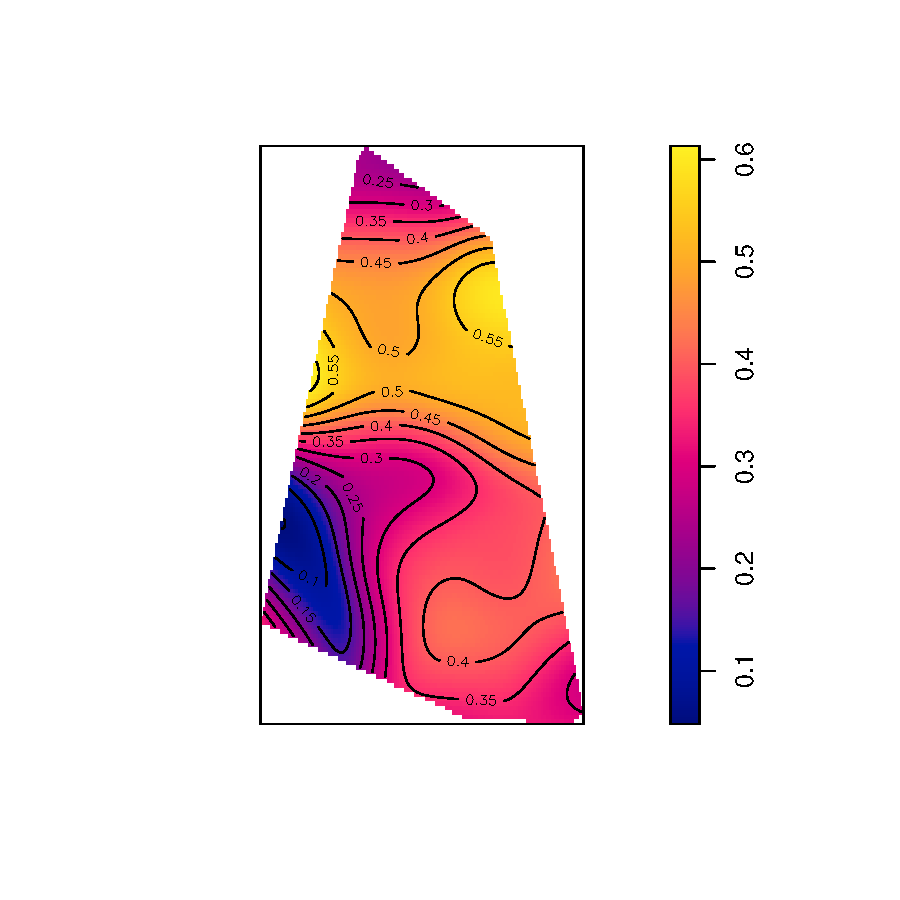
\includegraphics[width=0.7\textwidth]{graficos/canchayllo_risk_to_sampling.pdf}
	\caption{Riesgo de participar en la muestra en Canchayllo}
	\label{canchayllo_risk_to_sampling}
\end{figure}

\newpage

\begin{figure}[h]
	\centering
	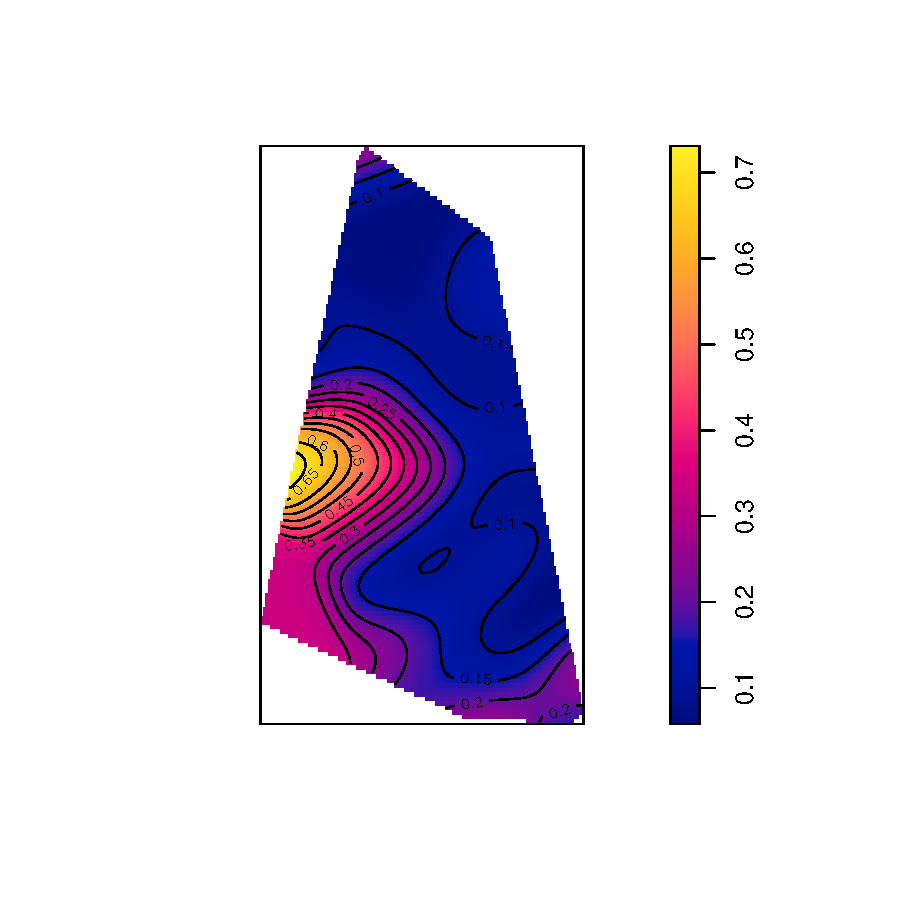
\includegraphics[width=0.7\textwidth]{graficos/canchayllo_risk_to_disease.pdf}
	\caption{Riesgo de la enfermedad en la muestra en Canchayllo}
	\label{canchayllo_risk_to_disease}
\end{figure}

\newpage

\subsection*{Ajuste del modelo}
Se seleccionó un modelo GAM usando los pesos obtenidos según la metodología propuesta. Se tomó como covariable a la tenencia de perros (Tener o no tener más de 3 perros). Este modelo tuvo un AUC de 0.664 y 0.763 para los datos de entrenamiento y prueba, respectivamente

\subsection*{Inferencia}

Tras haber hecho el ajuste correspondiente, se obtuvo una prevalencia corregida, la cual ascendió a 0.245. Asimismo, el riesgo espacial fue corregido, lo cual muestra una observable diferencia con el el riesgo antes de realiza la corrección. Además, se puede observar la zona en la que el riesgo se concentra.

\begin{figure}[h]
	\centering
	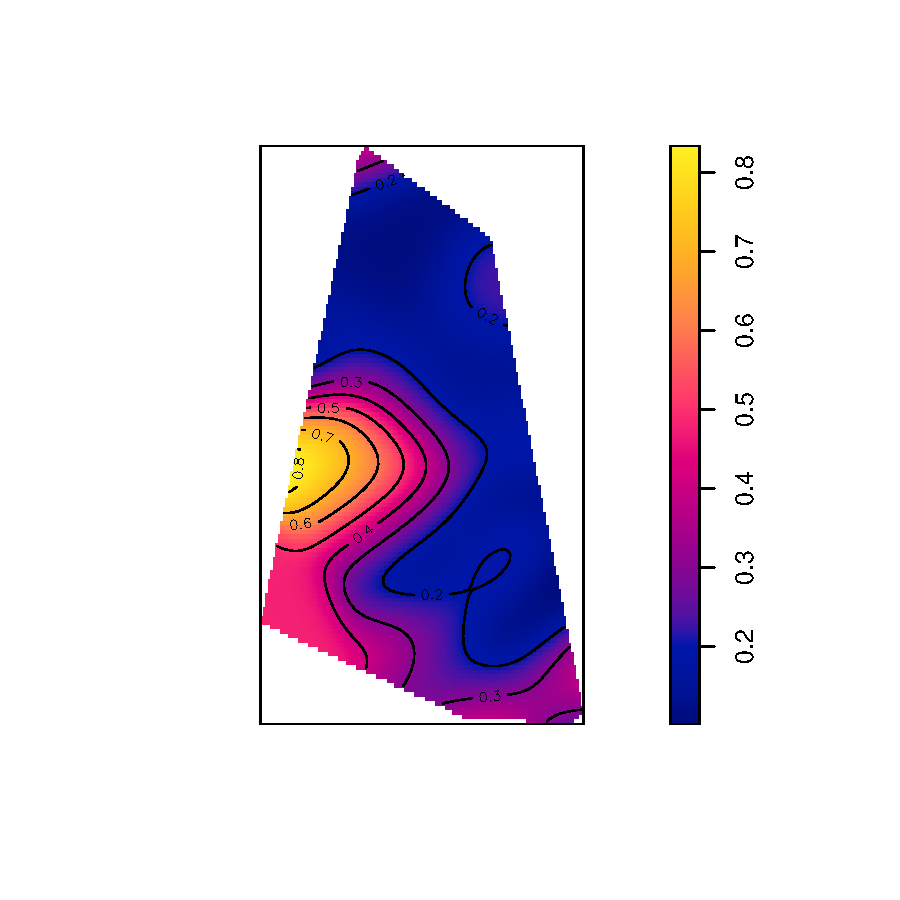
\includegraphics[width=0.7\textwidth]{graficos/canchayllo_risk_to_disease_fixed.pdf}
	\caption{Riesgo de la enfermedad en la muestra en Canchayllo}
	\label{canchayllo_risk_to_disease_fixed}
\end{figure}
